\documentclass[border=12pt]{standalone}
\def\pgfsysdriver{pgfsys-dvisvgm.def}
\usepackage[dvisvgm]{xcolor}
\usepackage{xeCJK}
\setCJKmainfont{HaranoAjiGothic-Regular.otf}[BoldFont=HaranoAjiGothic-Bold.otf]
\setCJKsansfont{HaranoAjiGothic-Regular.otf}[BoldFont=HaranoAjiGothic-Bold.otf]
\usepackage{amsmath,amssymb,tikz,lmodern}
\usetikzlibrary{arrows.meta,positioning,calc,fit,backgrounds}
\renewcommand{\familydefault}{\sfdefault}
\definecolor{ink}{HTML}{25322F}
\definecolor{green}{HTML}{246657}
\definecolor{tint}{HTML}{EEF4F0}
\definecolor{soft}{HTML}{C6D2CC}
\definecolor{muted}{HTML}{52615B}
\newif\ifJapanese
\newcommand{\Tx}[2]{\ifJapanese #1\else #2\fi}
\newcommand{\Eff}{\overline{\operatorname{Eff}}}
\newcommand{\heading}[3]{{\color{green}\bfseries #1\quad\Tx{#2}{#3}}\\[5pt]}
% A white rectangle makes the complete citation label clickable, including spaces.
\newcommand{\refurl}[2]{\special{dvisvgm:raw <a xlink:href="#1" target="_blank" rel="noopener noreferrer">}{\setlength{\fboxsep}{0pt}\colorbox{white}{\color{green}\underline{\strut #2}}}\special{dvisvgm:raw </a>}}
\newcommand{\refedge}[3]{\refurl{\csname source#1\endcsname\string##page=#2}{#3}}
\newcommand{\SF}[2]{\refedge{sf}{#1}{#2}}
% GitHub's file preview does not support PDF page fragments.
\newcommand{\LA}[2]{\refurl{\sourcela}{#2}}
\newcommand{\Sch}[2]{\refedge{sch}{#1}{#2}}
\newcommand{\PS}[2]{\refedge{ps}{#1}{#2}}
\tikzset{
 card/.style={draw=soft,fill=white,rounded corners=2pt,align=left,text=ink,font=\fontsize{10.5}{14}\selectfont,inner xsep=12pt,inner ysep=10pt,text width=14.4cm},
 half/.style={card,text width=6.45cm,minimum height=2.05cm},
 result/.style={card,draw=green,fill=tint,line width=.9pt},
 reason/.style={align=left,text=muted,font=\fontsize{9}{12}\selectfont,inner sep=0pt,text width=12.7cm},
 branchreason/.style={reason,text width=5.95cm},
 edge/.style={-{Stealth[length=2.4mm]},draw=green,line width=1pt},
 wire/.style={draw=green,line width=1pt},
}
% Keep the arrow in a dedicated left gutter; explanations never cover it.
\newcommand{\flow}[3]{
 \coordinate (#2-from) at ($(#1.south)+(-6.9,0)$);
 \coordinate (#2-to) at ($(#2.north)+(-6.9,0)$);
 \draw[edge] (#2-from)--(#2-to);
 \node[reason,anchor=west] (#2-reason) at ($(#2-from)!.5!(#2-to)+(.55,0)$) {#3};
}
\newcommand{\Cite}[2]{\refurl{\csname source#1\endcsname}{#2}}

\Japanesetrue
\newcommand{\sourceck}{https://github.com/openai/math/blob/adc7f1241b42e322a6451854ab7e4b4c146bf78a/preprints/Conditional-good-minimal-models-for-compact-Kahler-fourfolds-October-5-2026/paper.pdf}
\newcommand{\sourceoi}{https://github.com/openai/math/blob/adc7f1241b42e322a6451854ab7e4b4c146bf78a/preprints/Orbifold-and-logarithmic-Iitaka-subadditivity-September-26-2026/paper.pdf}
\newcommand{\sourcefm}{https://github.com/openai/math/blob/adc7f1241b42e322a6451854ab7e4b4c146bf78a/preprints/Finite-ordinary-minimal-model-programs-on-compact-Kahler-fourfolds-October-5-2026/paper.pdf}
\newcommand{\sourcean}{https://github.com/openai/math/blob/adc7f1241b42e322a6451854ab7e4b4c146bf78a/preprints/Abundance-after-nonvanishing-for-compact-Kahler-fourfolds-September-27-2026/paper.pdf}
\newcommand{\sourcedps}{https://arxiv.org/pdf/math/0006205v2}
\newcommand{\sourceou}{https://arxiv.org/pdf/2501.18088v1}
\newcommand{\sourcedo}{https://arxiv.org/pdf/2306.00671v4}
\newcommand{\sourcecce}{https://arxiv.org/pdf/1302.5016v3}
\begin{document}
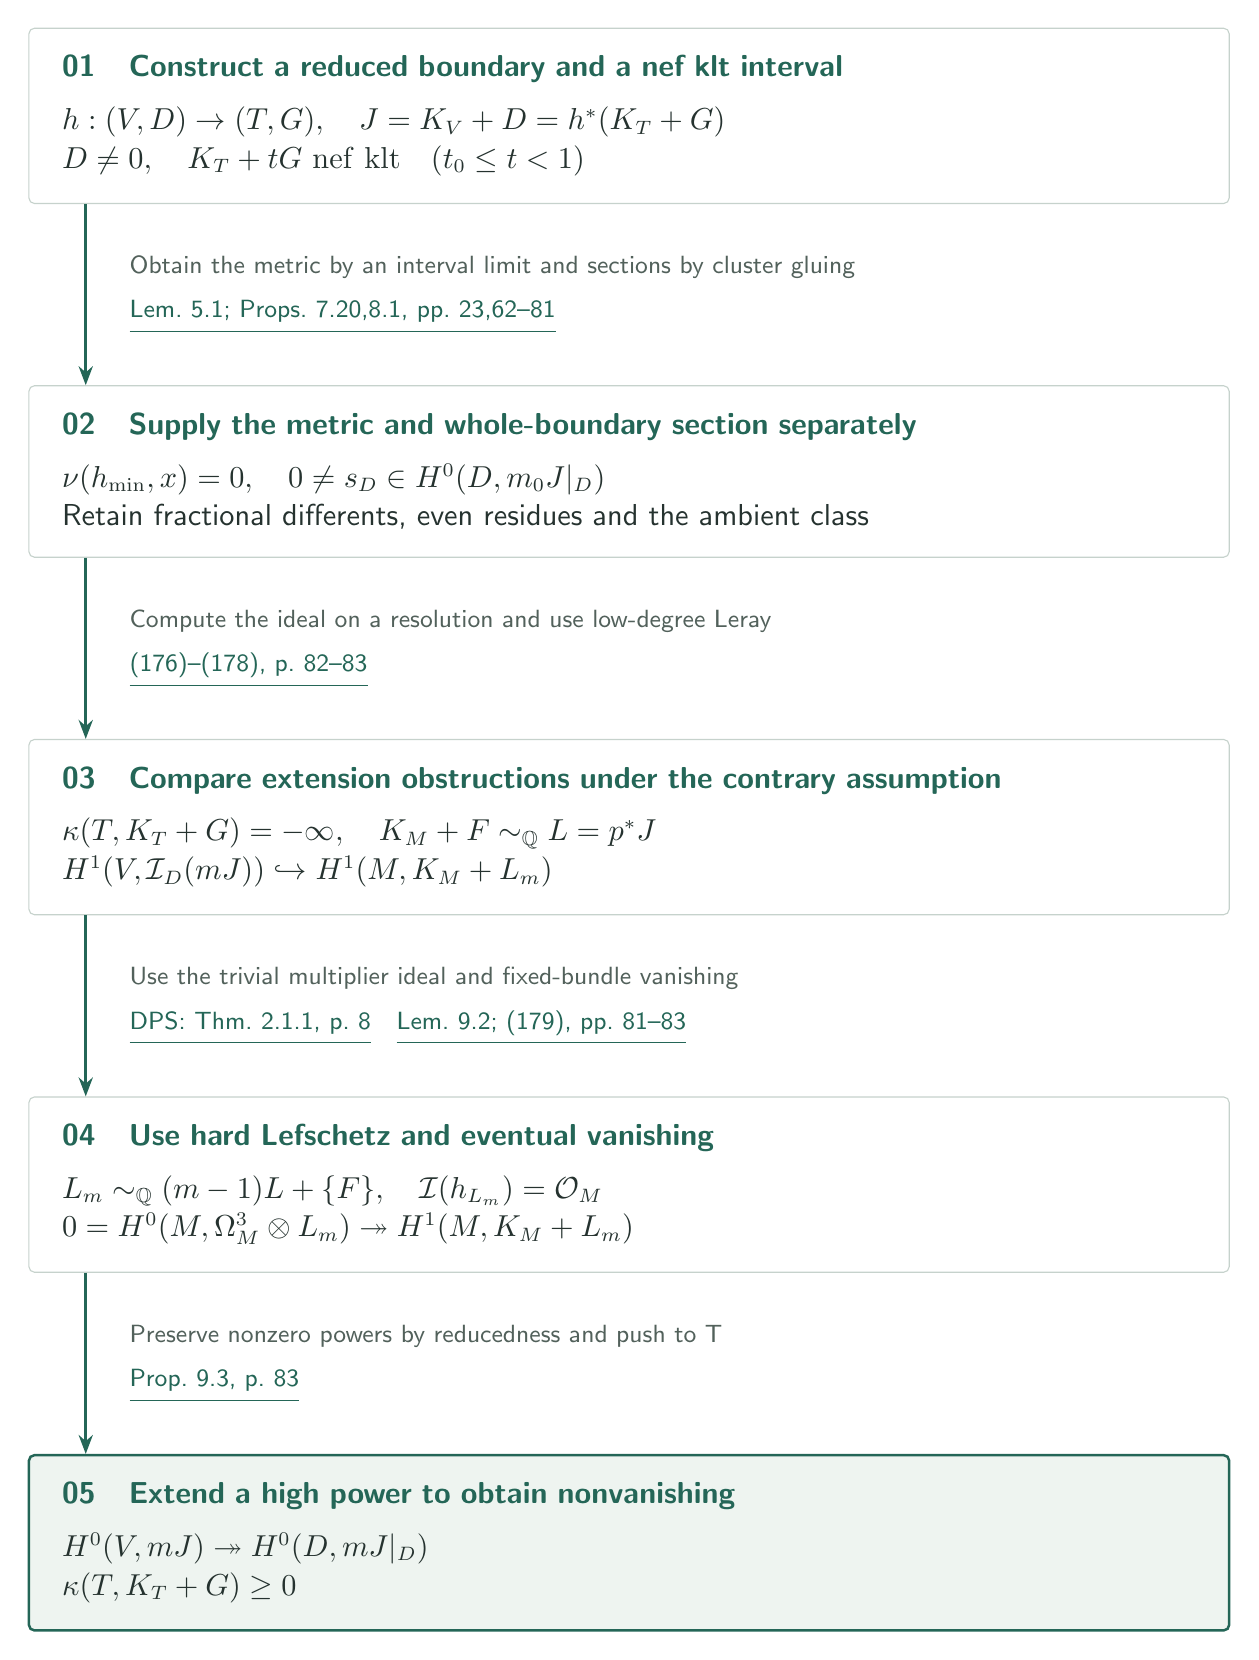
\begin{tikzpicture}
\node[card] (n0) {\heading{01}{reduced境界とnef klt区間を構成}{Construct a reduced boundary and a nef klt interval}\Tx{$h:(V,D)\to(T,G),\quad J=K_V+D=h^*(K_T+G)$\\$D\ne0,\quad K_T+tG\ {\rm nef\ klt}\quad(t_0\leq t<1)$}{$h:(V,D)\to(T,G),\quad J=K_V+D=h^*(K_T+G)$\\$D\ne0,\quad K_T+tG\ {\rm nef\ klt}\quad(t_0\leq t<1)$}};
\node[card,below=2.3cm of n0] (n1) {\heading{02}{計量と全境界の節を別々に用意}{Supply the metric and whole-boundary section separately}\Tx{$\nu(h_{\min},x)=0,\quad 0\ne s_D\in H^0(D,m_0J|_D)$\\分数different・偶数留数・ambient Kähler類を保持}{$\nu(h_{\min},x)=0,\quad 0\ne s_D\in H^0(D,m_0J|_D)$\\Retain fractional differents, even residues and the ambient class}};
\flow{n0}{n1}{\Tx{区間の極限で計量、clusterの貼合せで節を得る}{Obtain the metric by an interval limit and sections by cluster gluing}\\[4pt]\Cite{ck}{Lem.\ 5.1; Props.\ 7.20,8.1, pp.\ 23,62--81}}
\node[card,below=2.3cm of n1] (n2) {\heading{03}{反証仮定の下で延長障害を比較}{Compare extension obstructions under the contrary assumption}\Tx{$\kappa(T,K_T+G)=-\infty,\quad K_M+F\sim_{\mathbb Q}L=p^*J$\\$H^1(V,\mathcal I_D(mJ))\hookrightarrow H^1(M,K_M+L_m)$}{$\kappa(T,K_T+G)=-\infty,\quad K_M+F\sim_{\mathbb Q}L=p^*J$\\$H^1(V,\mathcal I_D(mJ))\hookrightarrow H^1(M,K_M+L_m)$}};
\flow{n1}{n2}{\Tx{解消で理想層を計算しlow-degree Lerayを使う}{Compute the ideal on a resolution and use low-degree Leray}\\[4pt]\Cite{ck}{(176)--(178), p.\ 82--83}}
\node[card,below=2.3cm of n2] (n3) {\heading{04}{hard Lefschetzとeventual vanishing}{Use hard Lefschetz and eventual vanishing}\Tx{$L_m\sim_{\mathbb Q}(m-1)L+\{F\},\quad\mathcal I(h_{L_m})=\mathcal O_M$\\$0=H^0(M,\Omega_M^3\otimes L_m)\twoheadrightarrow H^1(M,K_M+L_m)$}{$L_m\sim_{\mathbb Q}(m-1)L+\{F\},\quad\mathcal I(h_{L_m})=\mathcal O_M$\\$0=H^0(M,\Omega_M^3\otimes L_m)\twoheadrightarrow H^1(M,K_M+L_m)$}};
\flow{n2}{n3}{\Tx{自明なmultiplier idealと固定bundleの消滅}{Use the trivial multiplier ideal and fixed-bundle vanishing}\\[4pt]\Cite{dps}{DPS: Thm.\ 2.1.1, p.\ 8}\quad \Cite{ck}{Lem.\ 9.2; (179), pp.\ 81--83}}
\node[result,below=2.3cm of n3] (n4) {\heading{05}{高い冪を延長して非消滅へ}{Extend a high power to obtain nonvanishing}\Tx{$H^0(V,mJ)\twoheadrightarrow H^0(D,mJ|_D)$\\$\kappa(T,K_T+G)\geq0$}{$H^0(V,mJ)\twoheadrightarrow H^0(D,mJ|_D)$\\$\kappa(T,K_T+G)\geq0$}};
\flow{n3}{n4}{\Tx{被約性で非零の冪を保ち、Tへ押し下げる}{Preserve nonzero powers by reducedness and push to T}\\[4pt]\Cite{ck}{Prop.\ 9.3, p.\ 83}}
\end{tikzpicture}
\end{document}
